\section{Proposed Method}
\begin{frame}{Proposed Method}
\begin{columns}
\begin{column}{.5\textwidth}
\begin{itemize}
\item Sanh et al. (2019)\cite{Sanh2019} proposed DistilBERT as a smaller, faster, cheaper, lighter and distiled version of BERT.
\item By fine-tuning DistilBERT, we proposed a efficient model for Text Classfication.
\item The outputs of DistilBERT at token \texttt{[CLS]} is fed into a fully-connected layer with parameters $W \in \mathbb{R}^{D\times H}$ and $b \in \mathbb{R}^H$. In that, $D$ is the dimensionality of the output vector and H denotes the number of classes. Finally, to predict the label, the softmax layer is applied.
\end{itemize}

\end{column}

\begin{column}{.5\textwidth}
\begin{figure}[htp]
\centering
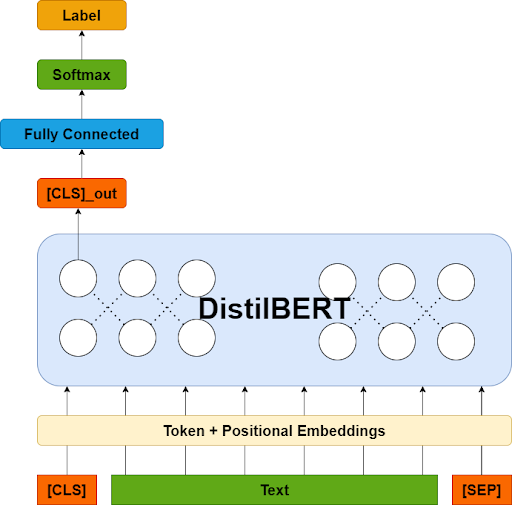
\includegraphics[scale=.3]{img/distilbert.png}
\caption{The overall architecture of our proposed method using DistilBERT.}
% \label{fig:distilbert}
\end{figure}
\end{column}
\end{columns}
\end{frame}